\documentclass{article}

\usepackage{graphicx}
\usepackage{hyperref}

\title{Yelp and Crime Data}  % TODO
\author{Kenneth Lin, Tom McCormick, Sid Naik}
\date{\today}

\begin{document}
\maketitle

\section{Problem Statement and Background}

For our CS 194 final project, we decided to investigate the potential
relationship between the City of San Francisco public safety data set and
the data set provided by the Yelp API. At first, we explored each data set
individually to discover general patterns in the data set. After that was
completed, we looked at the nearest 20 restaurants near each crime to see
if we could discover any common patterns of restaurants close to crimes.
% TODO problem statement

\subsection{City of San Francisco Public Safety Data Set}

-- introduction of data set
-- collection conditions

\begin{center}
  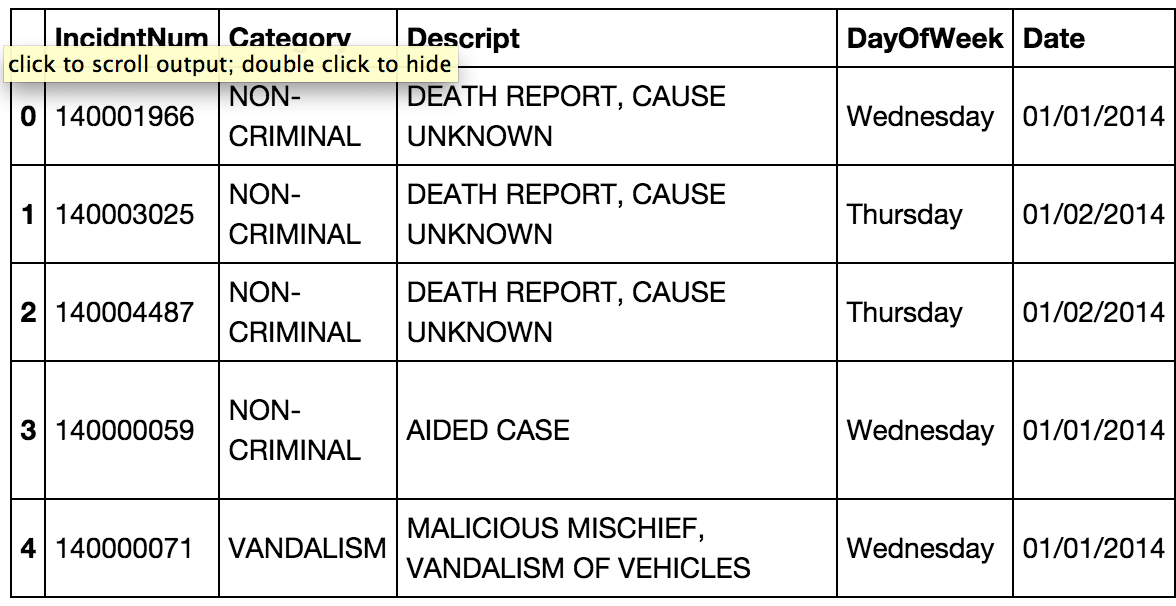
\includegraphics[scale=0.5]{sf_city_sample_1.png} \\
  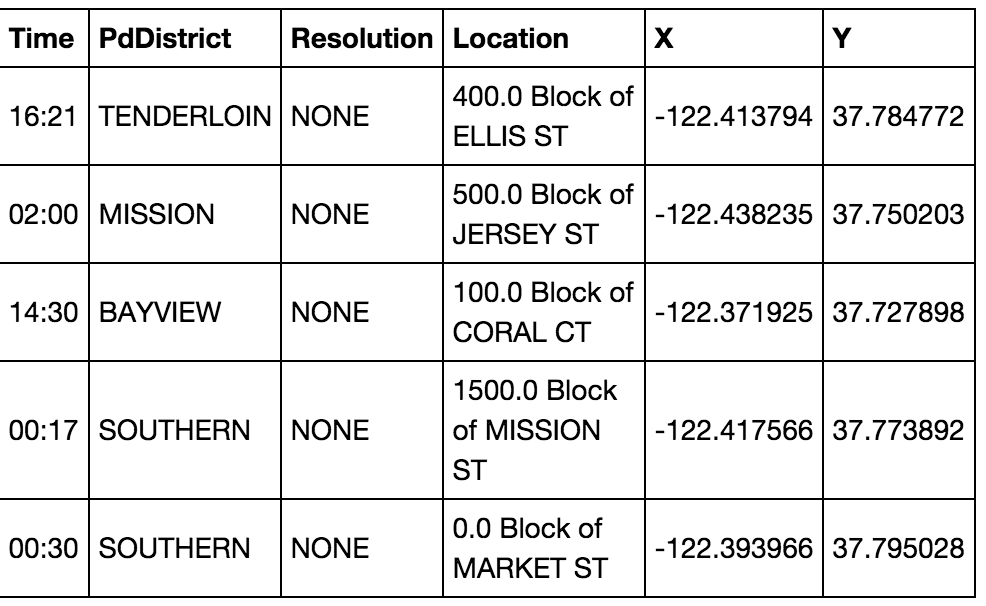
\includegraphics[scale=0.5]{sf_city_sample_2.png} \\
  Figure 1: Sample of San Francisco crime data set
\end{center}

The majority of the fields are self-explanatory. However, there are a few
things to note:
\begin{enumerate}
\item Category and descript are both categories, but category is more
  general. There are only 36 different ``Categories'' while there are 499
  different ``Descript''s in the year of 2014.
\item Resolution, though none are shown in the sample above, denote whether
  any action was taken and what that action was.
\item X denotes longitude, while Y denote latitude.
\end{enumerate}

A more detailed analysis is in the attached \texttt{analysis.ipynb}.

\subsection{Yelp Data Set}

Yelp.com is a platform which publishes crowd-sourced reviews about local
businesses. On Yelp, customers who have used the services of local
businesses may write reviews of these businesses and provide ratings of
their satisfaction. Reviewers may select from between 1 to 5 stars for each
review they make, and a business's average rating is the average of the
ratings of each of the reviews it has received. Yelp supplies a platform
for all kinds of local businesses ranging from restaurants to barbers to
museums; however, for the purpose of our research, we will look primarily
at restaurants as they are a very large majority of the reviews on Yelp.

There are two primary ways to access the data on Yelp. First, we can
utilize the search / business API
(\url{http://www.yelp.com/developers/documentation}). The search / business
API provides a way to search for local businesses matching a particular key
term (``restaurants'', for example) near a geographical location, and get
all the rating / review information about that restaurant. The API further
allows us to narrow the search to only the geographically closest
restaurants (not ranked by rating). This gives us a way to link the
geographical location of crime incidents to the types of restaurants near
that incident.

The other way of accessing Yelp data is through the academic data set
(\url{https://www.yelp.com/academic_dataset}). The Ylpe academic data set
provides all the data and associated reviews of the 250 closest businesses
for 30 universities, including UC Berkeley. Although not a random sample of
all businesses on Yelp, the academic data set provides a much better
estimate of all businesses in the Yelp data set population.

-- introduction of Yelp
-- two APIs
-- basic analysis

\subsection{Putting it together}

-- distribution
-- ratings

-- CONCLUSIONS??!?

-- map visualization problems
---- yelp data biased to near crime
---- not enough data on all of san francisco to create proper viz

-- condition tests in certain neighborhoods

\end{document}
